% Options for packages loaded elsewhere
\PassOptionsToPackage{unicode}{hyperref}
\PassOptionsToPackage{hyphens}{url}
%
\documentclass[
]{article}
\usepackage{amsmath,amssymb}
\usepackage{lmodern}
\usepackage{iftex}
\ifPDFTeX
  \usepackage[T1]{fontenc}
  \usepackage[utf8]{inputenc}
  \usepackage{textcomp} % provide euro and other symbols
\else % if luatex or xetex
  \usepackage{unicode-math}
  \defaultfontfeatures{Scale=MatchLowercase}
  \defaultfontfeatures[\rmfamily]{Ligatures=TeX,Scale=1}
\fi
% Use upquote if available, for straight quotes in verbatim environments
\IfFileExists{upquote.sty}{\usepackage{upquote}}{}
\IfFileExists{microtype.sty}{% use microtype if available
  \usepackage[]{microtype}
  \UseMicrotypeSet[protrusion]{basicmath} % disable protrusion for tt fonts
}{}
\makeatletter
\@ifundefined{KOMAClassName}{% if non-KOMA class
  \IfFileExists{parskip.sty}{%
    \usepackage{parskip}
  }{% else
    \setlength{\parindent}{0pt}
    \setlength{\parskip}{6pt plus 2pt minus 1pt}}
}{% if KOMA class
  \KOMAoptions{parskip=half}}
\makeatother
\usepackage{xcolor}
\IfFileExists{xurl.sty}{\usepackage{xurl}}{} % add URL line breaks if available
\IfFileExists{bookmark.sty}{\usepackage{bookmark}}{\usepackage{hyperref}}
\hypersetup{
  pdftitle={Reference-based OTU clustering for machine learning classification},
  hidelinks,
  pdfcreator={LaTeX via pandoc}}
\urlstyle{same} % disable monospaced font for URLs
\usepackage[margin=1.0in]{geometry}
\usepackage{graphicx}
\makeatletter
\def\maxwidth{\ifdim\Gin@nat@width>\linewidth\linewidth\else\Gin@nat@width\fi}
\def\maxheight{\ifdim\Gin@nat@height>\textheight\textheight\else\Gin@nat@height\fi}
\makeatother
% Scale images if necessary, so that they will not overflow the page
% margins by default, and it is still possible to overwrite the defaults
% using explicit options in \includegraphics[width, height, ...]{}
\setkeys{Gin}{width=\maxwidth,height=\maxheight,keepaspectratio}
% Set default figure placement to htbp
\makeatletter
\def\fps@figure{htbp}
\makeatother
\setlength{\emergencystretch}{3em} % prevent overfull lines
\providecommand{\tightlist}{%
  \setlength{\itemsep}{0pt}\setlength{\parskip}{0pt}}
\setcounter{secnumdepth}{-\maxdimen} % remove section numbering
\newlength{\cslhangindent}
\setlength{\cslhangindent}{1.5em}
\newlength{\csllabelwidth}
\setlength{\csllabelwidth}{3em}
\newlength{\cslentryspacingunit} % times entry-spacing
\setlength{\cslentryspacingunit}{\parskip}
\newenvironment{CSLReferences}[2] % #1 hanging-ident, #2 entry spacing
 {% don't indent paragraphs
  \setlength{\parindent}{0pt}
  % turn on hanging indent if param 1 is 1
  \ifodd #1
  \let\oldpar\par
  \def\par{\hangindent=\cslhangindent\oldpar}
  \fi
  % set entry spacing
  \setlength{\parskip}{#2\cslentryspacingunit}
 }%
 {}
\usepackage{calc}
\newcommand{\CSLBlock}[1]{#1\hfill\break}
\newcommand{\CSLLeftMargin}[1]{\parbox[t]{\csllabelwidth}{#1}}
\newcommand{\CSLRightInline}[1]{\parbox[t]{\linewidth - \csllabelwidth}{#1}\break}
\newcommand{\CSLIndent}[1]{\hspace{\cslhangindent}#1}
\usepackage{helvet}
\renewcommand*\familydefault{\sfdefault}
\usepackage{setspace}
\doublespacing
\usepackage[left]{lineno}
\usepackage{multirow}
\usepackage[none]{hyphenat}
\ifLuaTeX
  \usepackage{selnolig}  % disable illegal ligatures
\fi

\title{\textbf{Reference-based OTU clustering for machine learning
classification}}
\author{}
\date{\vspace{-2.5em}}

\begin{document}
\maketitle

\vspace{5mm}

Running title: Reference-based OTU clustering for ML classification

\vspace{10mm}

Courtney R. Armour\({^1}\), Kelly L. Sovacool\({^2}\), William L.
Close\(^{1,*}\), Begüm D. Topçuoğlu\(^{1,\#}\), Jenna Wiens\({^3}\),
Patrick D. Schloss \(^{1,\dagger}\)

\vspace{10mm}

\({^1}\) Department of Microbiology and Immunology, University of
Michigan, Ann Arbor, Michigan, USA

\({^2}\) Department of Computational Medicine and Bioinformatics,
University of Michigan, Ann Arbor, Michigan, USA

\({^3}\) Department of Electrical Engineering and Computer Science,
University of Michigan, Ann Arbor, Michigan, USA

\({^*}\) Current Affiliation: Bio-Rad Laboratories, Hercules,
California, USA

\({^\#}\) Current Affiliation: Bristol Myers Squibb, Summit, New Jersey,
USA

\(\dagger\) To whom correspondence should be addressed:
\href{mailto:pschloss@umich.edu}{\nolinkurl{pschloss@umich.edu}}

\vspace{10mm}

\textbf{observation format} (max 1200 words, 2 figures, 25 ref)

\newpage

\linenumbers

\hypertarget{abstract}{%
\subsection{Abstract}\label{abstract}}

Machine learning classification of disease based on the gut microbiome
often relies on clustering 16S rRNA gene sequences into operational
taxonomic units (OTUs) to quantify microbial composition. The abundance
of each OTU is then used to train a classification model. The standard
\emph{de novo} approach to clustering sequences into OTUs leverages the
similarity of the sequences to each other rather than to a reference
database. However, OTU assignments depend on the sequences in the data
set and therefore can change if new data are added. This lack of
stability complicates classification because in order to use the model
to classify additional samples, the new sequences must be reclustered
with the old data and the model must be retrained with the new OTU
assignments. The new reference-based clustering algorithm, OptiFit,
addresses this issue by fitting new sequences into existing OTUs. While
OptiFit can produce high quality OTU clusters, it is unclear whether
this method for fitting new sequence data into existing OTUs will impact
the performance of classification models. We used OptiFit to cluster
additional data into existing OTU clusters and then quantified model
performance in classifying a data set containing samples from patients
with and without colonic screen relevant neoplasia (SRN). We compared
the performance of this model to the standard procedure of \emph{de
novo} clustering all the data together. We found that both approaches
performed equally well in classifying SRNs. Moving forward, when OTUs
are used in classification problems, OptiFit can streamline the process
of classifying new samples by avoiding the need to retrain models using
reclustered sequences.

\hypertarget{importance}{%
\subsection{Importance}\label{importance}}

There is great potential for using microbiome data to non-invasively
diagnose people. One of the challenges with using classification models
based on the relative abundance of operational taxonomic units (OTUs) is
that 16S rRNA gene sequences are assigned to OTUs based on their
similarity to other sequences in the data set. If data are generated
from new patients seeking a diagnosis, then it would be necessary to
reassign sequences to OTUs and retrain the classification model. Yet
there is a desire to have a single, validated model that can be widely
deployed. To overcome this obstacle, we applied the OptiFit clustering
algorithm which fits new sequence data to existing OTUs and allows for
the reuse of a consistent model. A random forest machine learning model
deployed using OptiFit performed as well as the traditional reassignment
and retrain approach. This result indicates that there is potential for
developing deployable machine learning classification models based on
OTU relative abundance data.

\newpage

Gut community composition is useful as a resource for machine learning
classification of diseases, such as colorectal cancer
(\protect\hyperlink{ref-baxter2016}{1},
\protect\hyperlink{ref-zackular2014}{2}). Taxonomic composition of
microbial communities can be assessed using amplicon sequencing of the
16S rRNA gene, which is the input to classification models. Analysis of
16S rRNA gene sequence data generally relies on similarity-based
clustering of sequences into operational taxonomic units (OTUs). The
process of OTU clustering can either be reference-based or \emph{de
novo}. The quality of OTUs generated with reference-based clustering is
generally poor compared to those generated with \emph{de novo}
clustering (\protect\hyperlink{ref-westcott2015}{3}). While \emph{de
novo} clustering produces high-quality OTU clusters where sequences are
accurately grouped based on similarity thresholds, the resulting OTU
clusters depend on the sequences within the data set and the addition of
new data has the potential to redefine OTU cluster composition. The
unstable nature of \emph{de novo} OTU clustering complicates deployment
of machine learning models since integration of additional data requires
reclustering all the data and retraining the model. The ability to
integrate new data into a validated model without reclustering and
retraining could allow for deployment of a single model that new data
can be continually tested against. Recently, Sovacool \emph{et al}
introduced OptiFit, a method for fitting new sequence data into existing
OTUs (\protect\hyperlink{ref-sovacool2022}{4}). While OptiFit can
effectively fit new sequence data to existing OTU clusters, it is
unknown if the use of OptiFit will have an impact on classification
performance. Here, we tested the ability of OptiFit to cluster new
sequence data into existing OTU clusters for the purpose of classifying
disease based on gut microbiome composition.

We compared two approaches, one using all the data to generate OTU
clusters, and the other generating \emph{de novo} OTU clusters with a
portion of the data and then fitting the remaining sequence data to the
existing OTUs using OptiFit. In the first approach, all the 16S rRNA
sequence data was \emph{de novo} clustered into OTUs with the OptiClust
algorithm in mothur (\protect\hyperlink{ref-westcott2017}{5}). The
resulting abundance data was then split into training and testing sets,
where the training set was used to tune hyperparameters and ultimately
train the model. The testing set was then classified with the model and
the performance of the model was quantified (Figure 1A). However, with
this methodology, we would have to regenerate the OTU clusters and
retrain the model if we wanted to classify additional samples. The
OptiFit algorithm (\protect\hyperlink{ref-sovacool2022}{4}) addresses
this problem by enabling new sequences to be clustered into existing
OTUs. The OptiFit workflow is similar to the OptiClust workflow, where
the data was clustered into OTUs and used to tune hyperparameters and
ultimately train the model. Then, we used OptiFit to fit sequence data
of samples not part of the original data set into the existing OTUs, and
used the same model to classify the samples (Figure 1B). To test how the
model performance compared between these two approaches, we used a
publicly available data set of 16S rRNA gene sequences from stool
samples of healthy subjects (n = 261) as well as subjects with SRN
consisting of advanced adenoma and carcinoma (n = 229)
(\protect\hyperlink{ref-baxter2016}{1}). The data set was randomly split
into an 80\% train set and 20\% test set. For the standard OptiClust
workflow, the training and test sets were \emph{de novo} clustered
together into OTUs, then the resulting abundance table was split into
the training and testing set. For the OptiFit workflow, the train set
was clustered \emph{de novo} into OTUs, and the remaining test set was
fit to the OTU clusters using the OptiFit algorithm. For both workflows,
the abundance table of the train set was used to tune hyperparameters
and train a random forest model to classify SRN. The test set was
classified as either control or SRN using the trained models. To account
for variation, the data set was randomly split 100 times and the process
repeated for each of the 100 data splits. By comparing the model
performance of classifying the samples in the test data set between the
OptiFit and OptiClust algorithms, we quantified the impact of using
OptiFit on model classification performance.

We first examined the quality of the resulting OTU clusters from the two
algorithms using the Matthews correlation coefficient (MCC). The MCC
score was quantified by examining all pairs of sequences and assessing
whether they belonged together in an OTU based on their similarity
(\protect\hyperlink{ref-westcott2017}{5}). MCC scores range between
negative one and one. A score of negative one means none of the
sequences in an OTU are within the similarity threshold and any
sequences within the similarity threshold are not in an OTU together. An
MCC score of zero means the sequences are randomly clustered. An MCC
score of 1 means all sequences in an OTU are within the similarity
threshold and all sequence pairs within the similarity threshold are in
the same OTU. To ensure that OptiFit is appropriately integrating new
sequence data into the existing OTUs, we expected the MCC scores
produced by the OptiClust and OptiFit workflows to be similar. Since the
data was only clustered once in the OptiClust workflow there was only
one MCC score while the OptiFit workflow produced an MCC score for the
OTU clusters from each data split. Overall, the MCC scores were similar
between OptiClust (MCC = 0.884) and OptiFit (average MCC = 0.879,
standard deviation = 0.002). This indicated that OptiFit performed as
well as OptiClust when integrating new sequences into the existing OTUs.

After verifying that the quality of the OTUs was consistent between
OptiClust and OptiFit, we examined the model performance for classifying
samples in the held out test data set. To quantify model performance, we
used the OTU relative abundances from the training data from the
OptiClust and OptiFit workflows to train a model to predict SRNs. Using
the predicted and actual diagnosis classification, we calculated the
area under the receiver operating characteristic curve (AUROC) for each
data split to quantify model performance. During cross-validation (CV)
training, the model performance was equivalent between the two
algorithms (p-value = 0.13, OptiClust mean CV AUROC = 0.694, OptiFit
mean CV AUROC = 0.697; Figure 2A). The trained model was then deployed
to classify the samples of the test data as control or SRN. The
performance on the test data was equivalent between the two algorithms
(p-value = 0.63, OptiClust mean test AUROC = 0.709, OptiFit mean test
AUROC = 0.712; Figures 2B and 2C) indicating that new data could be fit
to existing OTU clusters without impacting model performance.

We tested the ability of OptiFit to integrate new data into existing
OTUs for the purpose of machine learning classification using OTU
relative abundance. A potential problem with using OptiFit is that any
sequences from the new samples that do not map to the existing OTU
clusters will be discarded, resulting in a possible loss of information.
Regardless, we demonstrated that OptiFit can be used to fit new sequence
data into existing OTU clusters and performs equally well in predicting
SRN compared to \emph{de novo} clustering all the sequence data
together. The ability to integrate data from new samples into existing
OTUs enables the deployment of a single machine learning model. Further
analysis is needed to determine the number of samples that are necessary
to build a robust model capable of classifying diverse samples. A robust
machine learning model could be implemented as part of a non-invasive
and low-cost aid in diagnosing SRN and other diseases.

\hypertarget{materials-and-methods}{%
\subsection{Materials and Methods}\label{materials-and-methods}}

\textbf{\emph{Data Set.}} Raw 16S rRNA gene sequence data isolated from
human stool samples was downloaded from NCBI Sequence Read Archive
(accession no. SRP062005) (\protect\hyperlink{ref-baxter2016}{1},
\protect\hyperlink{ref-edgar2011}{6}). This data set contains stool
samples from a total of 490 subjects. For this analysis, samples from
subjects identified in the metadata as normal, high risk normal, or
adenoma were categorized as ``normal'', while samples from subjects
identified as advanced adenoma or carcinoma were categorized as ``screen
relevant neoplasia'' (SRN). The resulting data set consisted of 261
normal samples and 229 SRN samples.

\textbf{\emph{Data Processing.}} The full data set was preprocessed with
mothur (v1.47) (\protect\hyperlink{ref-schloss2009}{7}) to join forward
and reverse reads, merge duplicate reads, align to the SILVA reference
database (v132) (\protect\hyperlink{ref-quast2013}{8}), precluster,
remove chimeras with UCHIME (\protect\hyperlink{ref-edgar2011}{6}),
assign taxonomy, and remove non-bacterial reads following the Schloss
Lab MiSeq standard operating procedure described on the mothur website
(\url{https://mothur.org/wiki/miseq_sop/}). 100 splits of the 490
samples were generated where 80\% of the samples (392 samples) were
randomly assigned to the training set and the remaining 20\% (98
samples) were assigned to the test set. Using 100 splits of the data
accounts for the variation that may be observed depending on the samples
that are in the training or test sets. Each sample was in the training
set an average of 80 times (standard deviation = 4.1) and the test set
an average of 20 times (standard deviation = 4.1).

The data was processed through two workflows. In the control workflow,
all the data was clustered together with OptiClust
(\protect\hyperlink{ref-westcott2017}{5}) to generate OTUs and the
resulting abundance tables were split into the training and testing
sets. In the experimental workflow, the preprocessed data was split into
the training and testing sets. The training set was clustered into OTUs
using OptiClust, then the test set was fit to the OTUs of the training
set using the OptiFit algorithm
(\protect\hyperlink{ref-sovacool2022}{4}). The OptiFit algorithm was run
with method open so that any sequences that did not map to the existing
OTU clusters would form new OTUs. For both pathways, the shared files
were sub-sampled to 10,000 reads per sample.

\textbf{\emph{Machine Learning.}} Machine learning using random forest
was conducted with the R package mikrompl (v 1.2.0)
(\protect\hyperlink{ref-topuxe7uoglu2021}{9}) to predict the diagnosis
(SRN or normal) for the samples in the test set for each data split. The
training set was preprocessed to normalize OTU counts (scale and
center), collapse correlated OTUs, and remove OTUs with zero variance.
The preprocessing from the training set was then applied to the test
set. Any OTUs in the test set that were not in the training set were
removed. P values comparing model performance were calculated as
previously described (\protect\hyperlink{ref-topuxe7uoglu2020}{10}). The
averaged ROC curves were plotted by taking the average and standard
deviation of the sensitivity at each specificity value.

\textbf{\emph{Code Availability.}} The analysis workflow was implemented
in Snakemake (\protect\hyperlink{ref-koster2012}{11}) . Scripts for
analysis were written in R (\protect\hyperlink{ref-R2020}{12}) and GNU
bash (\protect\hyperlink{ref-GNUbash}{13}). The software used includes
mothur v1.47.0 (\protect\hyperlink{ref-schloss2009}{7}), RStudio
(\protect\hyperlink{ref-RStudio2019}{14}), the Tidyverse metapackage
(\protect\hyperlink{ref-wickham2019}{15}), R Markdown
(\protect\hyperlink{ref-xie_r_2018}{16}), the SRA toolkit
(\protect\hyperlink{ref-noauthor_sra-tools_nodate}{17}), and conda
(\protect\hyperlink{ref-noauthor_anaconda_2016}{18}). The complete
workflow and supporting files required to reproduce this study are
available at:
\url{https://github.com/SchlossLab/Armour_OptiFitGLNE_XXXX_2021}

\hypertarget{acknowledgements}{%
\subsection{Acknowledgements}\label{acknowledgements}}

This work was supported through a grant from the NIH (R01CA215574).

\newpage

\hypertarget{references}{%
\subsection{References}\label{references}}

\setlength{\parindent}{-0.25in}
\setlength{\leftskip}{0.25in}

\noindent

\hypertarget{refs}{}
\begin{CSLReferences}{0}{1}
\leavevmode\vadjust pre{\hypertarget{ref-baxter2016}{}}%
\CSLLeftMargin{1. }
\CSLRightInline{\textbf{Baxter NT}, \textbf{Ruffin MT}, \textbf{Rogers
MAM}, \textbf{Schloss PD}. 2016. Microbiota-based model improves the
sensitivity of fecal immunochemical test for detecting colonic lesions.
Genome Medicine \textbf{8}:37.
doi:\href{https://doi.org/10.1186/s13073-016-0290-3}{10.1186/s13073-016-0290-3}.}

\leavevmode\vadjust pre{\hypertarget{ref-zackular2014}{}}%
\CSLLeftMargin{2. }
\CSLRightInline{\textbf{Zackular JP}, \textbf{Rogers MAM},
\textbf{Ruffin MT,I}, \textbf{Schloss PD}. 2014. The human gut
microbiome as a screening tool for colorectal cancer. Cancer Prevention
Research \textbf{7}:1112--1121.
doi:\href{https://doi.org/10.1158/1940-6207.CAPR-14-0129}{10.1158/1940-6207.CAPR-14-0129}.}

\leavevmode\vadjust pre{\hypertarget{ref-westcott2015}{}}%
\CSLLeftMargin{3. }
\CSLRightInline{\textbf{Westcott SL}, \textbf{Schloss PD}. 2015. De novo
clustering methods outperform reference-based methods for assigning 16S
rRNA gene sequences to operational taxonomic units. PeerJ
\textbf{3}:e1487.
doi:\href{https://doi.org/10.7717/peerj.1487}{10.7717/peerj.1487}.}

\leavevmode\vadjust pre{\hypertarget{ref-sovacool2022}{}}%
\CSLLeftMargin{4. }
\CSLRightInline{\textbf{Sovacool KL}, \textbf{Westcott SL},
\textbf{Mumphrey MB}, \textbf{Dotson GA}, \textbf{Schloss PD}. 2022.
OptiFit: An improved method for fitting amplicon sequences to existing
OTUs. mSphere \textbf{7}:e00916--21.
doi:\href{https://doi.org/10.1128/msphere.00916-21}{10.1128/msphere.00916-21}.}

\leavevmode\vadjust pre{\hypertarget{ref-westcott2017}{}}%
\CSLLeftMargin{5. }
\CSLRightInline{\textbf{Westcott SL}, \textbf{Schloss PD}. 2017.
OptiClust, an improved method for assigning amplicon-based sequence data
to operational taxonomic units. mSphere \textbf{2}:e00073--17.
doi:\href{https://doi.org/10.1128/mSphereDirect.00073-17}{10.1128/mSphereDirect.00073-17}.}

\leavevmode\vadjust pre{\hypertarget{ref-edgar2011}{}}%
\CSLLeftMargin{6. }
\CSLRightInline{\textbf{Edgar RC}, \textbf{Haas BJ}, \textbf{Clemente
JC}, \textbf{Quince C}, \textbf{Knight R}. 2011. UCHIME improves
sensitivity and speed of chimera detection. Bioinformatics
\textbf{27}:2194--2200.
doi:\href{https://doi.org/10.1093/bioinformatics/btr381}{10.1093/bioinformatics/btr381}.}

\leavevmode\vadjust pre{\hypertarget{ref-schloss2009}{}}%
\CSLLeftMargin{7. }
\CSLRightInline{\textbf{Schloss PD}, \textbf{Westcott SL},
\textbf{Ryabin T}, \textbf{Hall JR}, \textbf{Hartmann M},
\textbf{Hollister EB}, \textbf{Lesniewski RA}, \textbf{Oakley BB},
\textbf{Parks DH}, \textbf{Robinson CJ}, \textbf{Sahl JW}, \textbf{Stres
B}, \textbf{Thallinger GG}, \textbf{Van Horn DJ}, \textbf{Weber CF}.
2009. Introducing mothur: Open-source, platform-independent,
community-supported software for describing and comparing microbial
communities. Applied and Environmental Microbiology
\textbf{75}:7537--7541.
doi:\href{https://doi.org/10.1128/AEM.01541-09}{10.1128/AEM.01541-09}.}

\leavevmode\vadjust pre{\hypertarget{ref-quast2013}{}}%
\CSLLeftMargin{8. }
\CSLRightInline{\textbf{Quast C}, \textbf{Pruesse E}, \textbf{Yilmaz P},
\textbf{Gerken J}, \textbf{Schweer T}, \textbf{Yarza P}, \textbf{Peplies
J}, \textbf{Glöckner FO}. 2013. The SILVA ribosomal RNA gene database
project: Improved data processing and web-based tools. Nucleic Acids
Research \textbf{41}:D590--D596.
doi:\href{https://doi.org/10.1093/nar/gks1219}{10.1093/nar/gks1219}.}

\leavevmode\vadjust pre{\hypertarget{ref-topuxe7uoglu2021}{}}%
\CSLLeftMargin{9. }
\CSLRightInline{\textbf{Topçuoğlu BD}, \textbf{Lapp Z}, \textbf{Sovacool
KL}, \textbf{Snitkin E}, \textbf{Wiens J}, \textbf{Schloss PD}. 2021.
mikropml: User-Friendly R Package for Supervised Machine Learning
Pipelines. Journal of Open Source Software \textbf{6}:3073.
doi:\href{https://doi.org/10.21105/joss.03073}{10.21105/joss.03073}.}

\leavevmode\vadjust pre{\hypertarget{ref-topuxe7uoglu2020}{}}%
\CSLLeftMargin{10. }
\CSLRightInline{\textbf{Topçuoğlu BD}, \textbf{Lesniak NA},
\textbf{Ruffin MT}, \textbf{Wiens J}, \textbf{Schloss PD}. 2020. A
framework for effective application of machine learning to
microbiome-based classification problems. mBio \textbf{11}:e00434--20.
doi:\href{https://doi.org/10.1128/mBio.00434-20}{10.1128/mBio.00434-20}.}

\leavevmode\vadjust pre{\hypertarget{ref-koster2012}{}}%
\CSLLeftMargin{11. }
\CSLRightInline{\textbf{Koster J}, \textbf{Rahmann S}. 2012.
Snakemake--a scalable bioinformatics workflow engine. Bioinformatics
\textbf{28}:2520--2522.
doi:\href{https://doi.org/10.1093/bioinformatics/bts480}{10.1093/bioinformatics/bts480}.}

\leavevmode\vadjust pre{\hypertarget{ref-R2020}{}}%
\CSLLeftMargin{12. }
\CSLRightInline{\textbf{R Core Team}. 2020.
\href{https://www.R-project.org/}{R: A language and environment for
statistical computing}. R Foundation for Statistical Computing, Vienna,
Austria.}

\leavevmode\vadjust pre{\hypertarget{ref-GNUbash}{}}%
\CSLLeftMargin{13. }
\CSLRightInline{\textbf{GNU Project}.
\href{https://www.gnu.org/software/bash/\%20manual/bash.html/}{Bash
reference manual}.}

\leavevmode\vadjust pre{\hypertarget{ref-RStudio2019}{}}%
\CSLLeftMargin{14. }
\CSLRightInline{\textbf{RStudio Team}. 2019.
\href{http://www.rstudio.com/}{RStudio: Integrated development
environment for r}. RStudio, Inc., Boston, MA.}

\leavevmode\vadjust pre{\hypertarget{ref-wickham2019}{}}%
\CSLLeftMargin{15. }
\CSLRightInline{\textbf{Wickham H}, \textbf{Averick M}, \textbf{Bryan
J}, \textbf{Chang W}, \textbf{McGowan LD}, \textbf{François R},
\textbf{Grolemund G}, \textbf{Hayes A}, \textbf{Henry L}, \textbf{Hester
J}, \textbf{Kuhn M}, \textbf{Pedersen TL}, \textbf{Miller E},
\textbf{Bache SM}, \textbf{Müller K}, \textbf{Ooms J}, \textbf{Robinson
D}, \textbf{Seidel DP}, \textbf{Spinu V}, \textbf{Takahashi K},
\textbf{Vaughan D}, \textbf{Wilke C}, \textbf{Woo K}, \textbf{Yutani H}.
2019. Welcome to the Tidyverse. Journal of Open Source Software
\textbf{4}:1686.
doi:\href{https://doi.org/10.21105/joss.01686}{10.21105/joss.01686}.}

\leavevmode\vadjust pre{\hypertarget{ref-xie_r_2018}{}}%
\CSLLeftMargin{16. }
\CSLRightInline{\textbf{Xie Y}, \textbf{Allaire JJ}, \textbf{Grolemund
G}. 2018. R {Markdown}: {The Definitive Guide}. {Taylor \& Francis, CRC
Press}.}

\leavevmode\vadjust pre{\hypertarget{ref-noauthor_sra-tools_nodate}{}}%
\CSLLeftMargin{17. }
\CSLRightInline{{SRA}-{Tools} - {NCBI}.
http://ncbi.github.io/sra-tools/.}

\leavevmode\vadjust pre{\hypertarget{ref-noauthor_anaconda_2016}{}}%
\CSLLeftMargin{18. }
\CSLRightInline{2016. Anaconda {Software Distribution}. Anaconda
Documentation. Anaconda Inc.}

\end{CSLReferences}

\setlength{\parindent}{0in}
\setlength{\leftskip}{0in}

\newpage

\hypertarget{figures}{%
\subsection{Figures}\label{figures}}

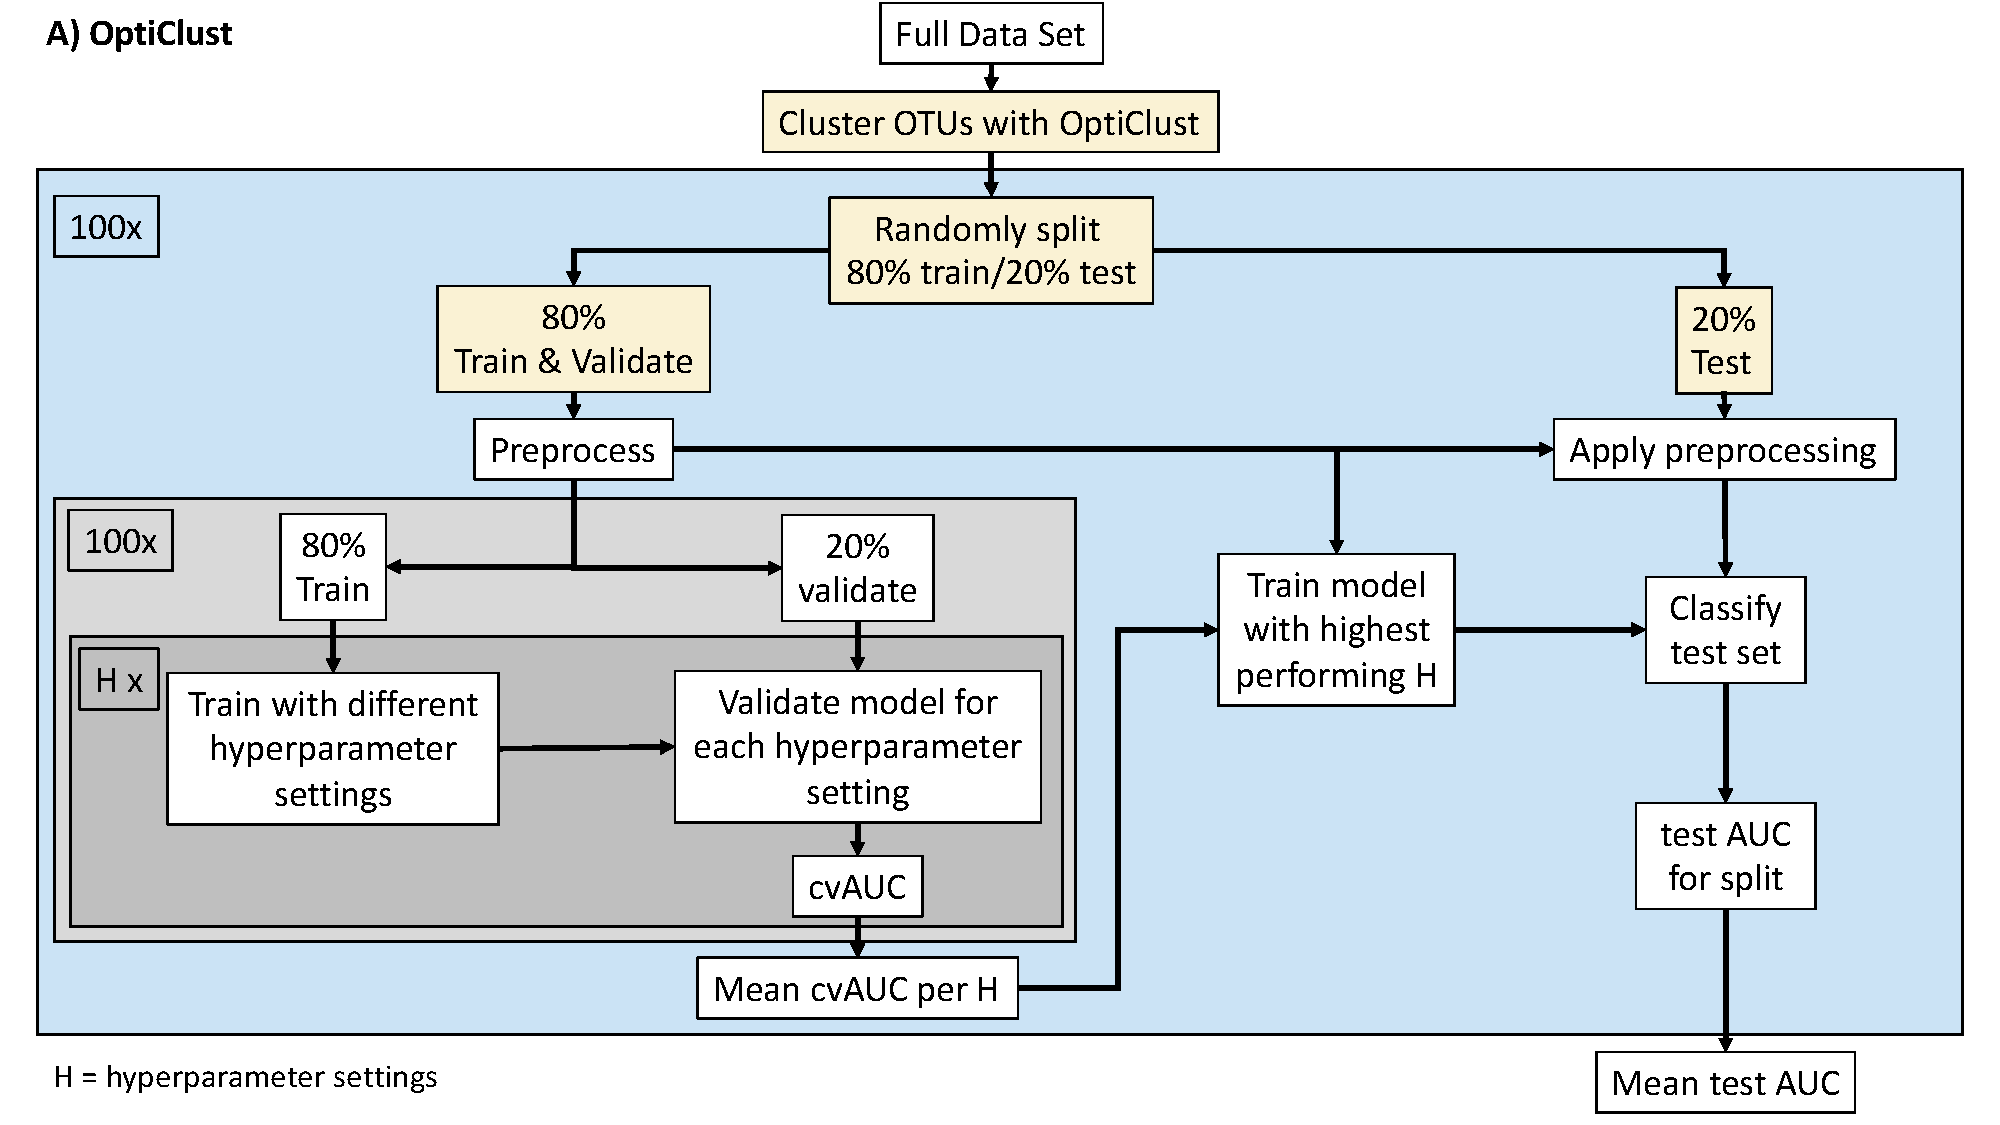
\includegraphics{../exploratory/figures/figure1_a.pdf}

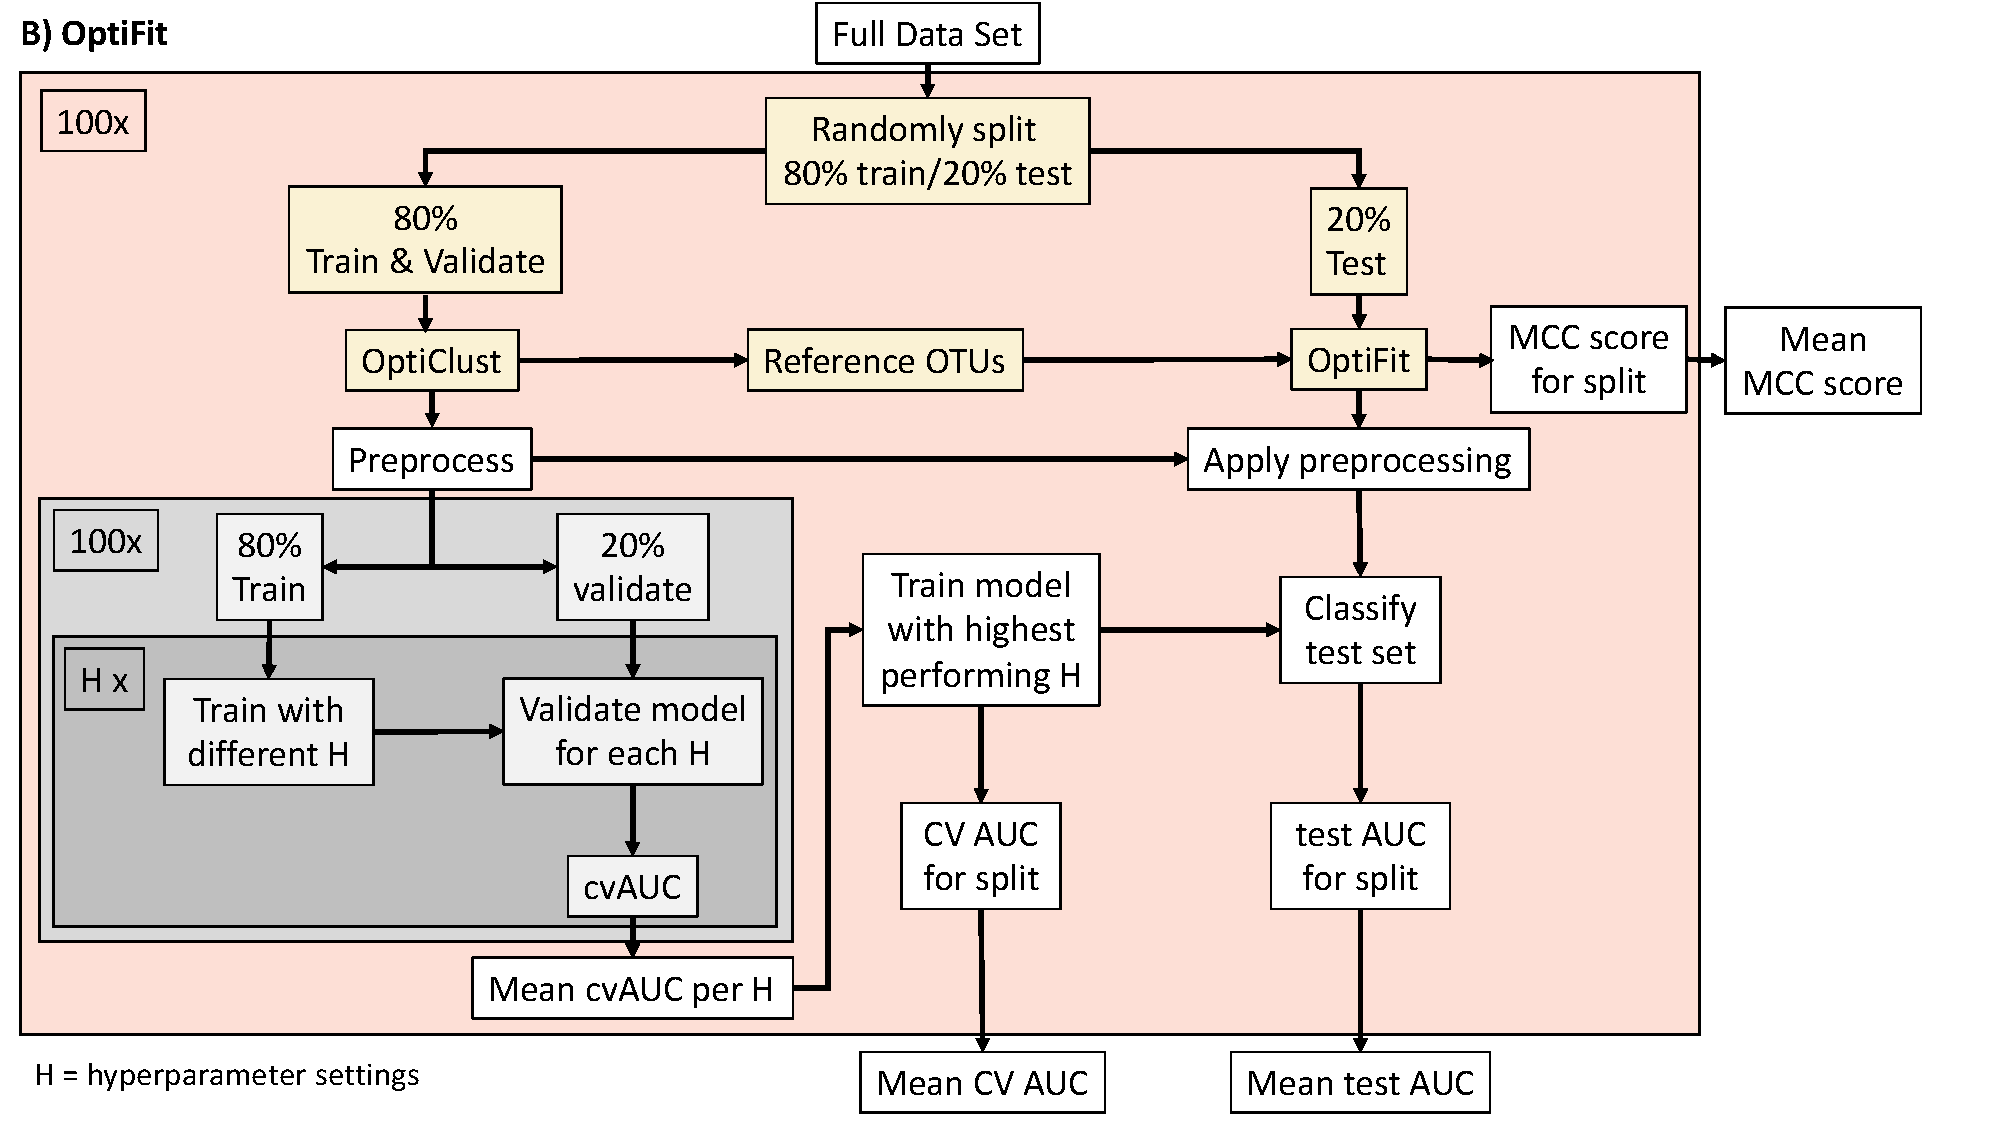
\includegraphics{../exploratory/figures/figure1_b.pdf}

\textbf{Figure 1: Workflows.} \textbf{A)} OptiClust workflow: The full
data set was clustered into OTUs using the OptiClust algorithm in
mothur. The data was then split into two sets where 80\% of the samples
were assigned to the training set and 20\% to the testing set. The
training set was preprocessed with mikropml to normalize values (scale
and center), collapse correlated features, and remove features with zero
variance. Using mikropml, the training set was split into train and
validate sets to compare results using different hyperparameter
settings. The highest performing hyperparameter setting was then used to
train the model with the full training set. The preprocessing scale from
the training set was applied to the test data set, then the trained
model was used to classify the samples in the test set. Based on the
actual classification and predicted classification, the area under the
receiver operating characteristic curve (AUROC) was calculated to
summarize model performance. The entire process was repeated 100 times
to account for variability depending on the split of the data resulting
in a total of 100 AUROC values summarizing the performance of the
standard OptiClust workflow. \textbf{B)} OptiFit workflow: The data set
was first split into two sets where 80\% of the samples were assigned to
the training set and 20\% to the testing set. The training set was then
clustered into OTUs using the OptiClust algorithm in mothur. The
resulting abundance data was preprocessed with mikropml to normalize
values (scale/center), collapse correlated features, and remove features
with zero-variance. Using mikropml, the training set was split into
train and validate sets to compare results using different
hyperparameter settings. The highest performing hyperparameter setting
was then used to train the model with the full training set. The OptiFit
algorithm in mothur was used to cluster the held out testing data set
using the OTUs of the training set as a reference. The preprocessing
scale from the training set was applied to the test data set, then the
trained model was used to classify the samples in the test set. Based on
the actual classification and predicted classification, the area under
the receiver operating characteristic curve (AUROC) was calculated to
summarize model performance. The entire process was repeated 100 times
to account for variability depending on the split of the data resulting
in a total of 100 AUROC values summarizing the performance of the new
OptiFit workflow.

\newpage

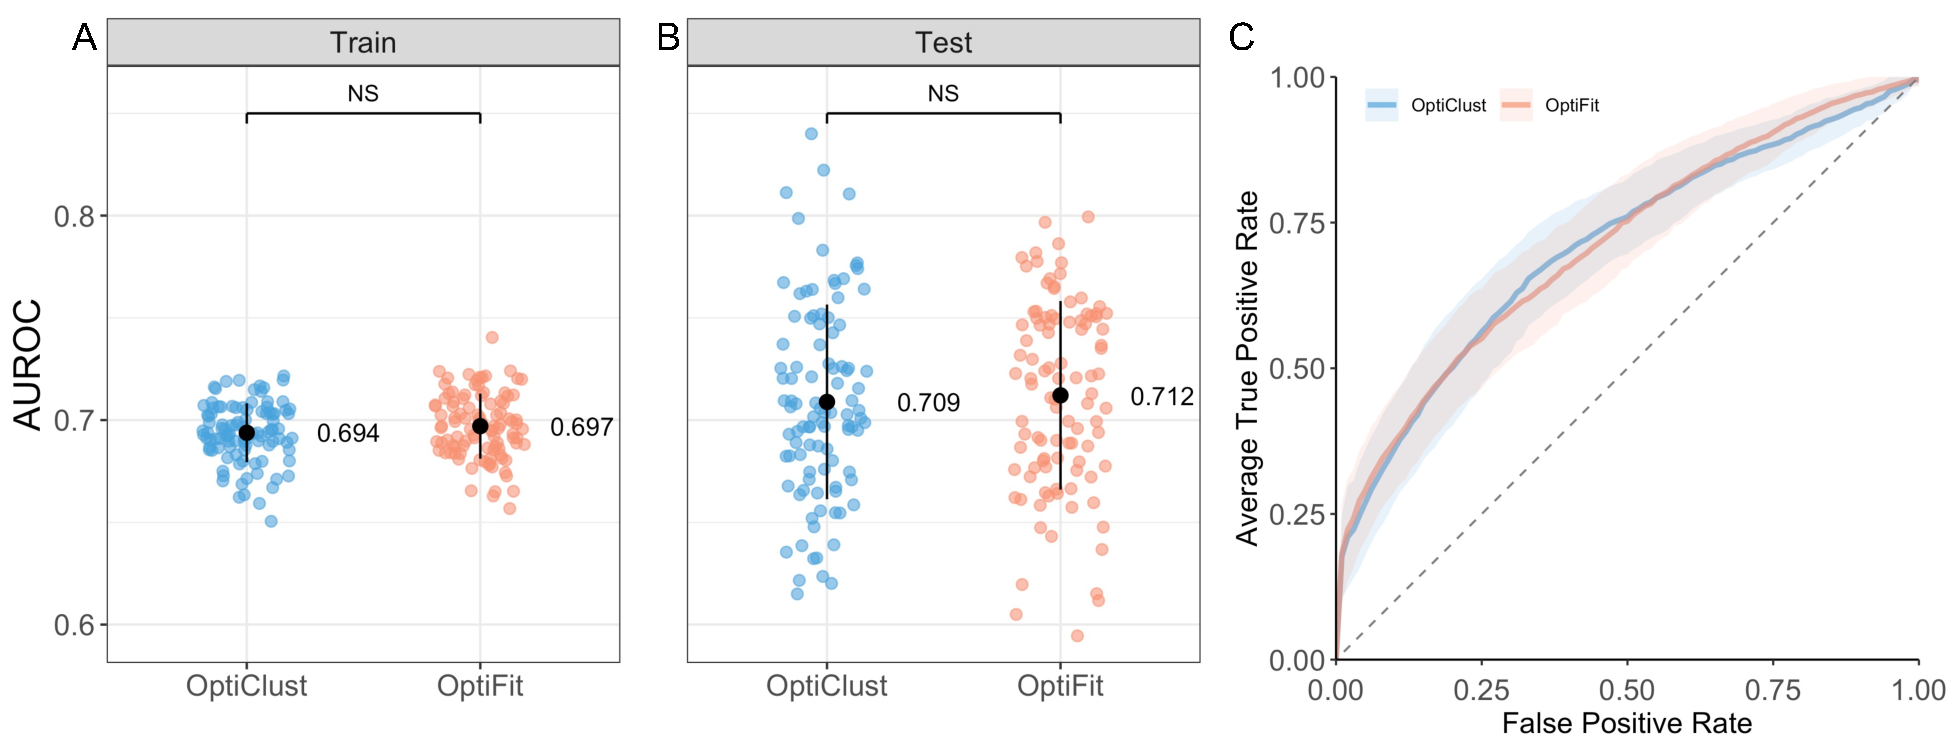
\includegraphics{../exploratory/figures/figure2.pdf}

\textbf{Figure 2: Model Performance.} \textbf{A)} Area under the
receiver operating characteristic (AUROC) curve during cross-validation
for the OptiClust and OptiFit workflows. Mean and standard deviation of
the AUROC is represented by the black dot and whiskers. Mean AUROC is
printed to the right of the points. \textbf{B)} AUROC on the test data
for the OptiClust and OptiFit workflows. Mean and standard deviation of
the AUROC is represented by the black dot and whiskers. The mean AUROC
is printed to the right of the points. \textbf{C)} Averaged receiver
operating characteristic (ROC) curves.

\end{document}
